\chapter{Comparazione dei principali tool open source esistenti}

\begin{epigraphs}
\qitem{"The mantra of any good security engineer is: 'Security is a not a product, but a process.' It's more than designing strong cryptography into a system; it's designing the entire system such that all security measures, including cryptography, work together."}{---\textsc{ Bruce Schneier, 'Applied Cryptography' author}}
\end{epigraphs}

Nel seguente capitolo verranno esposte le modalità di funzionamento di alcuni tool che eseguono analisi statica di codice PHP al fine di trovare vulnerabilità. Verranno confrontati gli approcci e verrà valutata la possibile applicabilità durante il normale ciclo di sviluppo software. \\
Alcuni di questi tool sono effettivamente disponibili, altri sono dei prototipi accademici, altri ancora non supportano le versioni più recenti di PHP. l'obiettivo di tale sezione è quello di illustrare come la ricerca di vulnerabilità tramite analisi statica di codice PHP non presenti soluzioni affermate e si cercherà di spiegarne le motivazioni.

\section{Pixy}
Pixy è un tool di analisi statica scritto in Java per la detection di vulnerabilità in codice PHP 4, rilasciato sotto licenza GPL. Sviluppato da Jovanovic\cite{pixy} come lavoro accademico, inizialmente consentiva la ricerca di sole vulnerabilità di tipo XSS ma successivamente è stato esteso alla ricerca di altre vulnerabilità di tipo taint-style, come SQL injections e command injections.\\
Pixy è flow sensitive, ovvero prende in considerazione l'ordine delle istruzioni del programma e la scansione che effettua è di tipo globale (interprocedural analysis), ovvero non valuta una funzione singolarmente ma tiene in considerazione il contesto in cui essa viene eseguita. Inoltre Pixy è dotato di un meccanismo di analisi degli alias che consente di ridurre i numerosi falsi positivi che tale caratteristica del linguaggio, quando utilizzata, potrebbe generare.\\
Pixy è disponibile anche in una versione web-based a funzionalità limitate sul sito ufficiale\cite{pixyweb}.

La scansione di Pixy si basa sulla definizione di tre parametri:
\begin{itemize}
\item \emph{Gli entry points del programma}: GET, POST e COOKIE.
\item \emph{Le funzioni di sanitizzazione}: htmlentities, htmlspecialchars ed opportuno type casting.
\item \emph{Sensitive sinks}: funzioni che ritornano output al browser, come print, echo, printf.
\end{itemize}
Queste definizioni sono stabilite tramite un file di configurazione in formato testuale.\\
L'obiettivo della scansione consiste nel determinare in quali circostanze è possibile che un dato tainted possa raggiungere un sensitive sink senza essere sanitizzato in modo opportuno. La tecnica per determinare ciò è quella della data-flow analysis, ovvero si computano in ogni punto del programma i possibili contenuti delle variabili per tracciare quali possono essere tainted. La data-flow analysis opera sul control flow graph del programma, quindi è necessario che prima dell'esecuzione venga costruito un albero (nello specifico un parse-tree) del file PHP in input. Tale operazione viene svolta con Jflex\cite{jflex}, un lexical analyzer scritto in java e Java Parser Cup\cite{jpc}, un generatore di parser in java.\\
Prima di eseguire la taint analysis sul control flow graph risultante vengono eseguite diverse operazioni, tra cui l'\emph{alias analysis}, che fornisce informazioni sugli alias, e la \emph{literal analysis}, che valuta le condizioni di branch ed esclude i percorsi che non possono essere eseguiti a run-time. Entrambe queste operazioni servono ad aumentare la precisione del tool, sebbene ne aumentino la complessità.\\
Pixy ignora le sanitizzazioni custom, generalmente effettuate con espressioni regolari, per due motivi: prima di tutto non è in grado di valutarle, cosa che è possibile solo con un'analisi dinamica, inoltre si ritiene a priori che effettuare sanitizzazioni mediante l'uso di espressioni regolari sia una pessima decisione implementativa a causa della facilità di errore.

La grossa problematica che affligge Pixy è data dal fatto che è stato abbandonato nel 2007, in questo momento non è in grado di parsare codice scritto secondo canoni moderni. Le ingenti modifiche apportate al linguaggio dalla release di PHP 5 hanno reso Pixy inadeguato per gli attuali progetti scritti in PHP.\\
La mancanza di una solida community ha fatto si che nessuna terza parte abbia forkato il progetto per proseguirne lo sviluppo, rendendolo ormai troppo datato.

Secondo i risultati dei test eseguiti dall'autore, Pixy ha una percentuale di falsi positivi che si aggira intorno al 50\%, soglia considerata dall'autore stesso accettabile per un tool di analisi statica su un linguaggio fortemente dinamico come PHP. Secondo le analisi eseguite da de Poel\cite{depoel} nel 2010, durante la scansione del codice sorgente di alcuni progetti open source viene dimostrato che Pixy non è in grado di funzionare con codebase recenti; la scansione ha infatti riportato risultati per solo cinque su sedici dei software analizzati e, neppure in questi casi, i risultati sono stati attendibili.
		
\section{Saner}
Saner è un prototipo, basato su Pixy, che combina le peculiarità di un'analisi statica con quelle di un'analisi dinamica. Sviluppato da Balzarotti et.al.\cite{saner} dimostra come sia possibile combinare i due approcci di analisi per migliorare i risultati ottenuti.\\
Saner esegue, in ordine, prima un'analisi statica sul sorgente, dopodiché procede con l'analisi dinamica di un data flow particolare. La parte di analisi statica viene eseguita da Pixy, che si occupa di determinare in che modo l'applicazione processa l'input, individuando eventuali sanitizzazioni mancanti o incomplete. Successivamente interviene una fase di analisi dinamica che si occupa di ricostruire il codice responsabile per la sanitizzazione dell'input. Una volta ricostruito, Saner processa tale codice con input malevoli per individuare eventuali problemi nelle sanitizzazioni.\\
Facendo affidamento sull'analisi dinamica, Saner è in grado di valutare eventuali sanitizzazioni custom al posto di reputarle direttamente come inaffidabili, cosa che il solo Pixy era costretto a fare.\\
Nell'esempio seguente viene evidenziato il valore del contributo dell'analisi dinamica nella scelta della giusta decisione da intraprendere.
Si suppone di dover analizzare il seguente codice:\\

\begin{lstlisting}[language=PHP]
$input = $_GET['x'];

$standard = htmlentities($input);
$standard = 'Hello' . $standard;
echo $standard;

$custom = str_replace('<', '', $input);
$custom = 'Hello' . $custom;
echo $custom;
\end{lstlisting}

Come Pixy, la maggior parte dei tool di analisi statica avrebbero marchiato la prima parte del codice riportato come safe a causa della presenza della funzione \emph{htmlentities}, che solitamente fa parte delle funzioni di sanitizzazione. Nel secondo caso però è presente una sanitizzazione custom costruita con la funzione \emph{str\_replace}. Siccome \emph{str\_replace} non fa parte delle funzioni di sanitizzazione, il codice viene marchiato come unsafe ed un warning viene riportato all'utente. Saner consente di eseguire tale sanitizzazione in modo dinamico sfruttando input appositamente malevoli al fine di verificare l'efficacia della sanitizzazione stessa, riducendo il numero di warning.\\
In un certo senso, Saner automatizza le operazioni che uno sviluppatore dovrebbe fare per verificare se un warning riportato da un tool di analisi statica è effettivamente una problematica di sicurezza.

I risultati riportati dall'autore dimostrano come la fase di analisi dinamica aumenti in modo elevato l'affidabilità del tool. Nell'analisi di cinque applicativi open-source di media complessità, Pixy segnala l'incapacità di determinare il valore della procedura di sanitizzazione per ben 66 sinks. Con l'ausilio dell'analisi dinamica è stato possibile determinare l'effettiva presenza di 14 vulnerabilità, mentre per i restanti 52 sinks l'analisi non è stata in grado di determinare dei valori di input che bypassassero la sanitizzazione.

\section{RIPS}
RIPS\cite{rips} è un tool per l'analisi statica di codice PHP rivolto alla ricerca di vulnerabilità sviluppato da Johannes Dahse.
E' l'unico tool open source scritto in PHP considerato usabile in sviluppo in data attuale.\\
Il tool è in grado di individuare vulnerabilità di tipo XSS, SQL Injection, file disclosure, code evaluation, remote command execution e busines logic flaw attraverso dei rule-sets definiti nei propri file di configurazione.\\
RIPS lavora in due fasi, costruzione del modello e analisi. Nella fase di costruzione del modello si possono individuare le operazioni di analisi semantica e lessicale, parsing e control flow analysis. Nella fase di analisi si individuano le operazione di taint analysis e local and global analysis.

La fase di analisi lessicale e semantica è caratterizzata dall'uso della libreria built-in \emph{tokenizer} per trasformare i costrutti del linguaggio in uno stream di tokens, attraverso l'uso della funzione \emph{token\_get\_all()} che trasforma ogni istruzione del linguaggio in un array costituito dal token, dal numero di riga dell'istruzione e dal codice originale. Successivamente vengono rimossi i tokens ritenuti inutili per l'analisi, come le spaziature ed il codice HTML, e trasformati alcuni tokens in equivalenti strutture più semplici da parsare (ad esempio vengono convertiti i costrutti di branches realizzati mediante la forma compatta in classici costrutti if-else).\\
La fase successiva, quella di parsing, avviene attraverso l'analisi dello stream di tokens, una sola volta per ogni file al fine di garantire migliori performance. In questa fase viene creata per ogni file una lista delle dipendenze e per alcuni costrutti vengono eseguite operazioni particolari. In caso di \emph{T\_INCLUDE} ad esempio lo stream di tokens del file da includere viene aggiunto allo stream corrente, in caso di \emph{T\_VARIABLE} viene controllato lo scope della variabile, ovvero se è una variabile globale o locale, e di conseguenza viene aggiunta ad una lista.\\
La fase di control flow analysis avviene in modo estremamente diverso da Pixy: se nel tool di Jovanovic si faceva riferimento al control flow graph, in RIPS la generazione dello stesso è stata evitata per problemi di performance. RIPS esegue la control flow analysis sfruttando la presenza di alcuni tokens come le parentesi graffe, \emph{T\_EXIT} e \emph{T\_THROW} che danno indicazioni sulle uscite da flussi di istruzioni.

La fase di analisi si basa sulle direttive definite attraverso array PHP nei file di configurazione. Tali direttive indicano gli input, i sinks, le funzioni di sanitizzazione con i rispettivi parametri da tracciare ed i token da ignorare.\\
RIPS cerca chiamate a funzioni, controlla se la funzione trovata è nella lista dei sinks ed in caso affermativo valuta i parametri di tale funzione. Una volta individuati i parametri rilevanti controlla nelle liste precedentemente create di variabili globali e locali se tali possono essere o meno tainted. In caso affermativo viene riportata la potenziale vulnerabilità.\\
RIPS è in grado di determinare se una funzione definita dall'utente è un sink. Nel caso in cui ciò accada infatti l'algoritmo può risalire ai parametri di input e quindi comprendere se il sink è determinato da uno di essi. In caso affermativo oltre alla funzione stessa anche le chiamate vengono trattate come un sink.

RIPS possiede una interfaccia web configurabile che consente di lanciare la scansione e che riporta i risultati. Tale interfaccia consente di definire per quale tipologia di vulnerabilità effettuare la scansione, il livello di verbosity e se comprendere le sottodirectory o meno. Il report dei risultati è dettagliato, vengono mostrate le linee di codice sorgente che riportano problematiche comprensive di motivazione, è possibile visualizzare un grafico delle chiamate che devono essere effettuate per raggiungere un certo sink e viene utilizzata la syntax highlighting per mostrare le linee di codice coinvolte.

Nei test effettuati alla Ruhr-University Bochum su una piattaforma ad uso interno, RIPS è stato in grado di esaminare 16870 linee di codice in 84 files, per un totale di 181 funzioni in 2.3 secondi. Nei risultati sono stati individuati diversi falsi positivi, dovuti all'uso di espressioni regolari per la sanitizzazione, metodologia non contemplata nell'analisi effettuata da RIPS, ed all'uso di fwrite per scrivere su file di testo. A seconda del livello di verbosity utilizzato varia il numero di falsi positivi riscontrati, poichè vengono incluse nei risultati delle vulnerabilità sospette ma non verificate.

RIPS è un tool che ben si adatta all'analisi statica per la ricerca di vulnerabilità. E' veloce, è configurabile con diversi livelli di verbosità, possiede una semplice e comprensibile interfaccia per il report dei risultati e produce un basso numero di falsi positivi.\\
Sebbene possieda le classiche limitazioni dei tool di analisi statica, come l'incapacità di valutare stringhe generate a run-time nel caso di inclusioni dinamiche di files o nel caso di chiamate dinamiche a funzioni che ne riducono l'accuratezza, l'estrema velocità rende adatto il suo utilizzo all'interno nel ciclo di sviluppo software.
RIPS è un tool in sviluppo ed attualmente non supporta completamente la semantica di PHP, ad esempio alcuni costrutti particolari come variabili di variabili o l'aliasing. Inoltre non supporta i costrutti tipici di PHP 5, ma supporta solo in modo basilare la dichiarazione di classi, oggetti e metodi.

L'approccio proposto da un tool come RIPS è estremamente differente da quello proposto da Pixy. RIPS è stato implementato con l'obiettivo di essere veloce e di riportare in modo chiaro i risultati, spiegando come una vulnerabilità funziona al posto di semplicemente specificare la linea in cui essa si trova, Pixy invece possiede un meccanismo di scansione più accurato ed ha come obiettivo il riuscire a riportare il minor numero di falsi positivi in assoluto.

\chapter{Vulture}
Vulture\cite{vulture} è un prototipo di tool per analisi statica volta alla ricerca di vulnerabilità di applicazioni web, progettato in collaborazione con EURECOM durante lo svolgimento di questo lavoro di tesi.\\
Nato inizialmente con l'obiettivo di produrre un sistema in grado di rilevare vulnerabilità di tipo Http Parameter Pollution server side, è stato generalizzato al fine di costruire una piattaforma estensibile, alla quale lo sviluppatore può aggiungere i propri insiemi di regole.\\
Inizialmente si è pensato di lavorare all'estensione di un tool esistente, in modo da aggiungere solo la parte di codice riguardante Http Parameter Pollution. Purtroppo però i candidati, analizzati in precedenza in questo documento, presentavano problematiche di progettazione rilevanti, che non potevano essere risolte facilmente ma avrebbero comportato la riscrittura di grosse porzioni del tool stesso. 
Le caratteristiche individuate come fondamentali erano le seguenti:
\begin{itemize}
\item Supporto a PHP 5
\item Possibilità di modifica della codebase
\item Estensibilità
\item Velocità di scansione
\item Basso numero di falsi positivi
\item Supporto
\item Scritto in PHP
\end{itemize}
La possibilità di modifica della codebase implicava che il tool fosse open source, gli unici due tools opensource rilevanti sono Pixy e RIPS.
Pixy non supporta però PHP 5, non è supportato dall'autore o da una community, non presenta una rilevante velocità di scansione ma è in grado di riportare un basso numero di falsi positivi grazie al supporto agli alias.
RIPS invece non supporta gli alias, caratteristica non molto utilizzata in PHP, e non fornisce come Pixy pieno supporto a classi, metodi ed oggetti, introdotti da PHP 5. Nonostante ciò è veloce e supportato dall'autore, caratteristiche fondamentali per la scelta di un tool sul quale lavorare.\\
Purtroppo però la codebase di RIPS si è rivelata decisamente problematica da estendere e modificare, il codice sorgente in formato procedurale con funzioni da migliaia di righe poco commentate hanno reso di fatto più semplice la riscrittura del tool rispetto al refactoring del codice esistente. Oltretutto RIPS possiede un approccio all'analisi basato sulla funzione tokenizer di PHP, ritenuta ad un livello troppo basso, ovvero troppo vicino al codice sorgente per l'analisi statica.

La soluzione ideale è stata individuata in un tool in grado di generare e parsare l'abstract syntax tree del codice sorgente, ottenendo una rappresentazione ad alto livello sulla quale effettuare la scansione. Il tool deve essere veloce, estensibile affinché sia possibile per uno sviluppatore aggiungere delle regole personalizzate per la ricerca di vulnerabilità. Quest'ultima caratteristica porta ad una considerazione: il tool verrà usato per trovare vulnerabilità nel codice sorgente scritto in PHP, quindi da sviluppatori che normalmente lavorano con tale linguaggio. Se si vuole che il tool venga poi esteso dalla community, difficilmente si potrà attenere un riscontro se lo scrive in un linguaggio diverso da PHP, proprio perché le competenze di chi lo userà sono focalizzate su quel linguaggio.\\

Vulture è un tool scritto in PHP dotato di un'interfaccia web. Non necessita di database e l'unico requisito per utilizzarlo è un web server. Il tool è basato su Symfony 2\cite{symfony}, un framework per la realizzazione di applicazioni web scritto in PHP da Fabien Potencier. Tale scelta è stata effettuata poiché tale framework fornisce le più comuni caratteristiche di un'applicazione web, come il meccanismo di routing delle pagine e la separazione tra logica e presentazione.\\
L'utilizzo di Symfony 2 non comporta un overhead per la visualizzazione delle pagine ed evita che si debba reinventare la ruota per problematiche già affrontate e di scarso interesse ai fini dello sviluppo del tool di analisi statica.

Vulture si presenta con una schermata\ref{vultureinizio} nella quale viene richiesto di inserire il percorso alla directory contenente il codice sorgente da analizzare. 

\begin{figure}[!h]
\centering
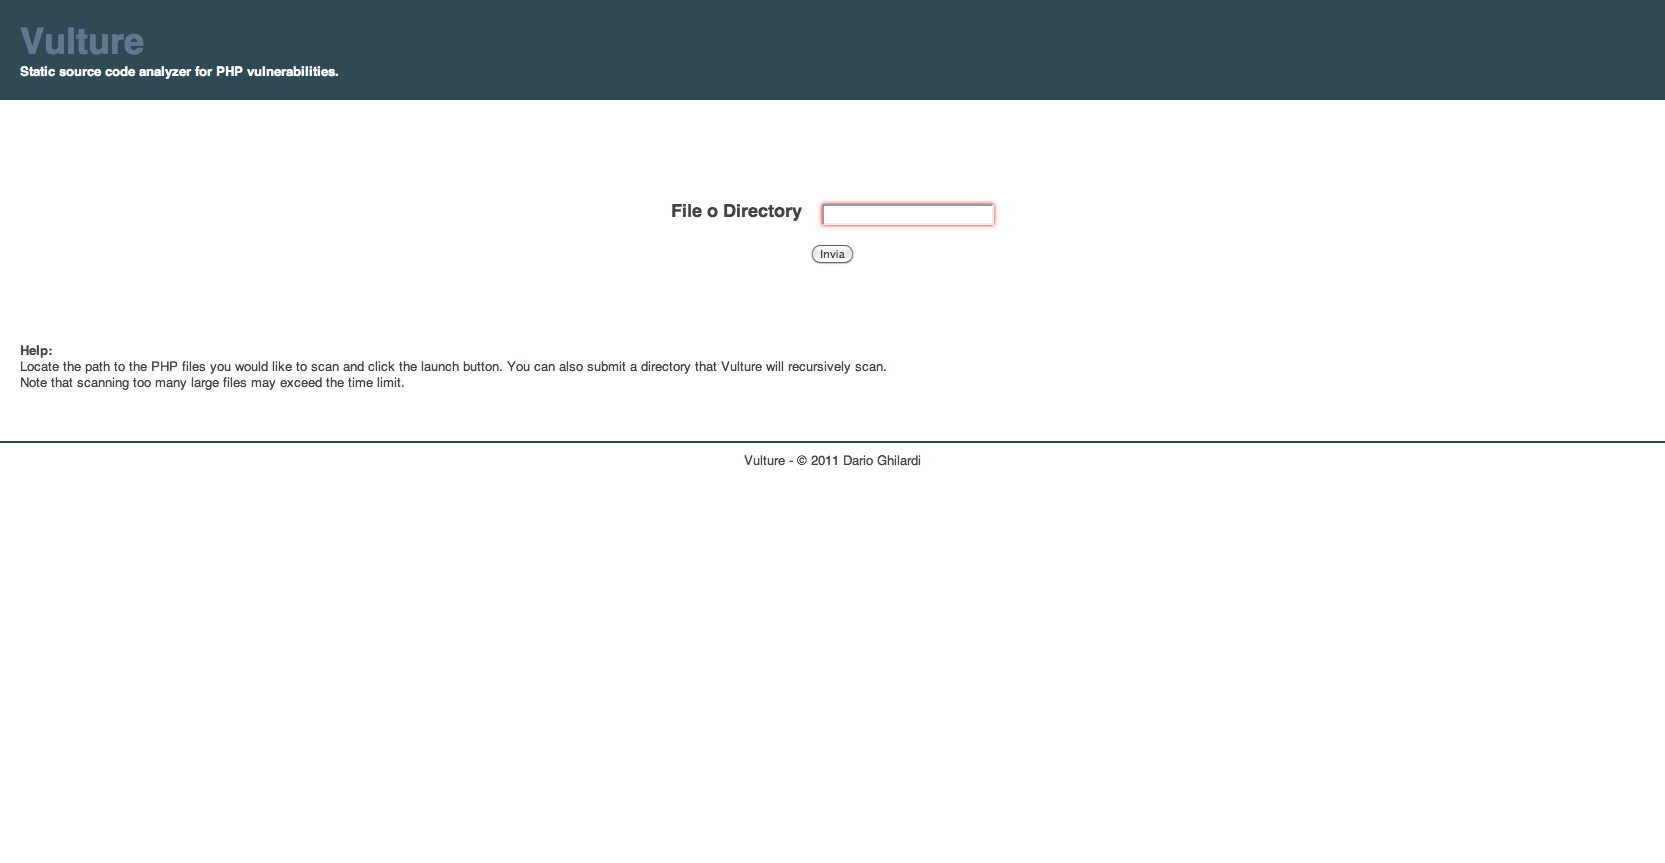
\includegraphics[width=16cm]{Vulture.png}
\caption{Vulture - Schermata iniziale}\label{vultureinizio}
\end{figure}

Ogni file viene esaminato in tale directory, sottodirectory comprese.\\
Successivamente il tool genera un AST del codice sorgente fornito in input. La generazione dell'AST avviene per mezzo di un progetto open source sperimentale chiamato PHP-Parser\cite{phpparser}. Sebbene in fase alfa, è attualmente l'unico strumento scritto in PHP in grado di generare un AST di codice sorgente che supporta tutte le caratteristiche dell'attuale release di PHP. \\
Esistono soluzioni alternative abbandonate o incomplete, come php-sat\cite{phpsat}, fermo dal 2006, o PHP\_Depend\cite{phpdepend}, che comprende un parser attualmente incompleto.
\newpage
L'output di PHP-Parser è una rappresentazione ad alto livello del codice sorgente, sotto forma di una combinazione di array ed oggetti. \\
Sono stati effettuati alcuni test per determinare l'efficacia di PHP-Parser: la scansione completa della codebase di Symfony2 funziona correttamente e richiede circa 35 secondi, un ottimo risultato viste le dimensioni della codebase in esame.\\

\begin{lstlisting}
array(
    0: Stmt_Echo(
        exprs: array(
            0: Scalar_String(
                value: This is 
                a php code example.<br />
                isBinary: false
                type: 1
            )
        )
    )
    1: Stmt_Echo(
        exprs: array(
            0: Expr_ArrayDimFetch(
                var: Variable(
                    name: _SERVER
                )
                dim: Scalar_String(
                    value: PHP_SELF
                    isBinary: false
                    type: 0
                )
            )
        )
    )
    2: Stmt_Echo(
        exprs: array(
            0: Expr_Concat(
                left: Scalar_String(
                    value: And this is a GET variable
                    : 
                    isBinary: false
                    type: 1
                )
                right: Expr_ArrayDimFetch(
                    var: Variable(
                        name: _GET
                    )
                    dim: Scalar_String(
                        value: p
                        isBinary: false
                        type: 0
                    )
                )
            )
        )
    )
\end{lstlisting}

Dopo la generazione dell'AST, si utilizza una metodologia di traversing dello stesso, identificando gli elementi utili a seconda della vulnerabilità che si sta cercando. Per determinare quali essi siano si usano i bundle di Symfony: la definizione di un nuovo bundle con una determinata struttura di files viene riconosciuta automaticamente come la definizione di un set di regole per la ricerca di una nuova vulnerabilità.\\
Ogni bundle costruito per Vulture consente la definizione di un set di input, un set di sinks ed un set di funzioni di sanitizzazione. E' su questi tre parametri che Vulture basa la sua scansione, in modo similare a quanto eseguito da RIPS.
 
Durante la scansione Vulture salva in memoria le variabili che vengono a contatto con valori tainted, ovvero alle quali vengono assegnati valori provenienti dall'input. Tali variabili vengono custodite in un array, che viene aggiornato ad ogni istruzione processata con le eventuali nuove variabili che divengono tainted a causa di assegnamenti. Se si incontra una funzione di sanitizzazione applicata su una variabile di tipo tainted, Vulture rimuove la variabile dall'array. Se invece si incontra un sink con una variabile presente nell'array tainted Vulture segnala una nuova vulnerabilità. Al fine di poter determinare se una funzione di sanitizzazione è efficace non basta che si identifichi la variabile come parametro della stessa, occorre conoscere anche in quale parametro viene posizionata: le funzioni in PHP sono state definite senza una cognizione, capita che il parametro sul quale viene applicata la funzione sia in prima posizione in alcuni casi, in seconda in altri. Per tale motivo è necessario definire un vocabolario di funzioni con le rispettive posizioni per i parametri in input, al fine di poter determinare se il parametro è posizionato o meno nel punto corretto per la sanitizzazione. Questo caos è una delle caratteristiche che hanno contribuito a ritenere PHP un linguaggio poco strutturato e l'hanno portato ad essere valutato negativamente dalle community di sviluppatori di altri linguaggi\cite{codinghorror}.\\
Quando vengono incontrate delle inclusioni, Vulture apre il file collegato e lo include nel flusso corrente costruendo un flusso unico continuo sul quale eseguire la scansione.

Attualmente il tool non è usabile e completo. Costruire un tool di analisi statica da zero è un problema complesso che non poteva essere risolto unicamente nel solo corso di questa tesi. Tool come RIPS e Pixy hanno richiesto anni di sviluppo (per la precisione RIPS è in sviluppo da 3 anni, Pixy è stato in sviluppo per altrettanti), e sono comunque loro stessi incompleti per quanto riguarda il supporto a classi, oggetti ed ai restanti costrutti di PHP 5.
Nonostante ciò sono state progettate le fasi successive per lo sviluppo di Vulture:

\begin{itemize}
\item \emph{Loop e branches}: Vulture non supporterà loop e branches al fine di rendere la scansione più veloce possibile.
\item \emph{Sanitizzazioni custom}: Vulture non supporterà sanitizzazioni custom, frutto ad esempio di espressioni regolari. Sarà però flessibile, in quanto consentirà la definizione manuale di funzioni di sanitizzazione, utile nel caso in cui si utilizzino dei framework che forniscono funzioni aggiuntive oltre a quelle del linguaggio. E' ovviamente un arma a doppio taglio, definire una funzione errata come sanitizzazione custom può risultare disastroso quindi occorre la massima cautela.
\item \emph{Inclusioni e chiamate a funzioni dinamiche}: Vulture, come tutti i tools di analisi statica, non è in grado di valutare inclusioni o chiamate a funzioni dinamiche. In questo caso verrà riportata una segnalazione.
\item \emph{Aliasing delle variabili}: L'aliasing delle variabili non è una caratteristica molto utilizzata in PHP. Realizzare un sistema in grado di valutare l'applicazione di tale funzionalità nell'analisi statica è molto complesso, ed il valore di ritorno sarebbe comunque basso, valido solo per le applicazioni che sfruttano tale caratteristica. Per tali ragioni lo sviluppo di tale funzionalità è stato posticipato.
\item \emph{Definizioni di classi e metodi e relative chiamate}: Il supporto a PHP 5 non è stato attualmente realizzato da alcun tool. Vulture si pone questo obiettivo per avere il pieno supporto alle applicazioni PHP moderne. L'idea alla base della realizzazione di tale funzionalità consiste nel trattare in modo particolare le classi con tutta una serie di accorgimenti, senza snaturare il funzionamento del tool. Sarà prevista una libreria di supporto che si occuperà di riconoscere i costrutti tipici delle classi e dei relativi oggetti e metodi.
\end{itemize}

Oltre alle caratteristiche analizzate fin'ora, PHP 5.3, un'ulteriore evoluzione del linguaggio, ha introdotto alcune novità come i namespace, le closures ed il late static binding. Tali strutture non sono attualmente previste nell'implementazione di Vulture ma sono senza dubbio fondamentali affinchè diventi possibile effettuare la scansione di moderne applicazioni web. Per tale motivo questo è una delle problematiche su cui sarà importante concentrarsi in futuro.

\chapter{Discussione}
In questo lavoro di tesi sono state analizzate dal punto di vista implementativo le principali soluzioni open source per l'esecuzione di analisi statica rivolta alla ricerca di vulnerabilità in applicazioni web. Esistono ovviamente anche soluzioni commerciali, tra le quali HP Fortify Static Code Analyzer\cite{fortify} ed Armorize CodeSecure\cite{codesecure}. Questi due prodotti non sono rivolti esclusivamente all'analisi di codice sorgente scritto in PHP ma ognuno di essi supporta molteplici linguaggi. Entrambi i tool sono stati confrontati nell'eccellente lavoro di analisi dei risultati svolto da Nico de Poel\cite{depoel}.\\
E' da notare come i tool open source non abbiano catturato un'audience rilevante. Sebbene il lavoro per la realizzazione sia tutt'altro che indifferente, i programmatori PHP hanno dimostrato scarso interesse per questo genere di tool, perlomeno non sufficiente per la nascita di una community di supporto. Ciò è senza dubbio la concausa dell'abbandono di tool promettenti come Pixy, insieme al mancato supporto per PHP 5.\\
Generalmente questa è la situazione che si verifica con tool che nascono in ambito accademico, i quali inizialmente raccolgono interesse, ma poi vengono abbandonati dai loro autori quando sono costretti a spostarsi verso altri topic di ricerca. Il risultato porta ad avere molti approcci diversi e molti prototipi, ma alla fine nessun prodotto sufficientemente valido per essere usato in produzione.\\
Per quanto riguarda i tool commerciali, non è possibile determinare la validità dell'approccio utilizzato poiché sono a sorgente chiuso. De Poel ha eseguito un'ottima comparazione basandosi sui risultati ottenuti dai tool open source e da quelli commerciali derivandone che i prodotti commerciali sono gli unici maturi sul mercato per questa tipologia di analisi.\\
E' importante però sottolineare come le carenze in questo ambito non siano da imputare solamente ai tool presenti sul mercato. La problematica maggiore è certamente la scarsa educazione degli sviluppatori alle problematiche di sicurezza. Se un numero maggiore di sviluppatori usasse questa tipologia di tool nel loro ciclo di sviluppo software, probabilmente tool come Pixy non sarebbero attualmente abbandonati, ma avrebbero raggiunto un grado di sviluppo eccellente per il problema che ambiscono a risolvere.\\
La questione si può riconoscere in una mancanza di tipo formativo, non tutti gli sviluppatori possiedono conoscenze sufficienti a sviluppare software sicuro; allo stesso modo non sono solitamente richieste certificazioni che determinino la conoscenza o meno delle problematiche di sicurezza nel software per uno sviluppatore. Si potrebbe formare maggiormente il personale, con evidenti costi da affrontare e responsabilità aggiuntive da stabilire, oppure assegnare a terzi il lavoro di code review. Quest'ultima soluzione è la più applicata, ma porta ad un ciclo di sviluppo software sbilanciato, in cui una vulnerabilità viene segnalata in un momento tardivo dello stesso sviluppo, aumentandone i costi di correzione.\\
Se le esigenze economiche sono da sempre la priorità, appare incomprensibile la mancanza di tool specifici che approccino questa problematica durante lo sviluppo software. E' per questo possibile ritenere che ci sia un enorme fetta di mercato scoperta per un possibile tool di analisi statica con i predetti scopi, perché è un'esigenza che le software house possiedono, ma di cui effettivamente sembrano non accorgersi.
  

\chapter{Conclusioni}
L'analisi statica finalizzata alla ricerca di vulnerabilità è una tecnologia promettente per ridurre le problematiche di sicurezza nelle applicazioni web moderne. La velocità di esecuzione consente l'integrazione di tale tecnica all'interno del ciclo di sviluppo software, facilitando il riconoscimento di vulnerabilità ed annullando la finestra di esposizione in quanto si va a sostituire il meccanismo di riconoscimento a posteriori con un sistema di integrazione continua. Ciò contribuisce anche ad abbassare i costi di gestione grazie all'immediata risposta fornita dal tool.
Per tali motivi l'analisi statica, sebbene imprecisa, può aggiungersi alla review del codice e fornire un grosso contributo nello sviluppo di applicazioni web sicure.\\
La creazione di un tool di analisi statica non è però un compito semplice, specialmente per linguaggi estremamente dinamici come PHP. L'impossibilità di valutare i tipi di dato, le inclusioni dinamiche e le chiamate a funzioni dinamiche sono solo alcune delle problematiche che non è possibile risolvere con la sola analisi statica e che influiscono pesantemente sui risultati delle scansioni.\\
Nonostante queste evidenti limitazioni, il settore dell'analisi statica è un ramo quasi inesplorato ed estremamente promettente, che potrebbe fare la fortuna di chi si dedicherà alla produzione del primo tool in grado di supportare i costrutti di PHP 5 e potrebbe essere un enorme passo avanti in una community di sviluppatori da sempre poco attenti alle problematiche di security.